\documentclass{article}
\usepackage[utf8]{inputenc}
\usepackage{geometry}
\usepackage{graphicx}
\usepackage{pgfplots}
\usepackage{amsmath}
\usepackage{amssymb}
\usepackage{amsfonts}
\usepackage{mdframed}
\usepackage{amsthm}
\usepackage{tikz}
\usepackage{multicol}
\usepackage{cancel}

\pgfplotsset{compat=1.18}
\geometry{a4paper, left=2cm, right=2cm, top=1cm, bottom=2cm}

\begin{document}
\begin{minipage}{0.7\textwidth}
    \small \textbf{COMPUTACIÓN PARA FÍSICOS, GRUPO 8106}  \\
    \small {Facultad de Ciencias, Universidad Nacional Autónoma de México} \\
    \small {Profesor: Francisco Ruiz Sala (\texttt{fruiz@astro.unam.mx})} \\
    \small {Ayudante: Manuel Silva Hernández (\texttt{masilher@ciencias.unam.mx})} \\
    \small {Fecha de entrega: 8 de Diciembre de 2023} \\
    \small {Nombre completo: Andrés López González} \\
    \small {Presentación formal del proyecto}
\end{minipage}
\hfill
\begin{minipage}{0.12\textwidth}
    
\includegraphics[width=\linewidth]{logo_universidad}
\end{minipage}


\section*{Descripción del problema.}

Este anteproyecto aborda la investigación de un fenómeno físico que implica un plano inclinado (37.5°) con un resorte en su base. El objetivo es analizar el movimiento de un objeto arrojado desde una altura específica respecto al resorte, siendo esta otorgada por el usuario, utilizando ecuaciones del resorte, cinemática y dinámica en general, además de poder visualizar una consecuencia directa del teorema trabajo-energía representando gráficamente las diversas energías de este sistema adiabático ideal: energía potencial del resorte, energía potencial gravitacional y energía cinética.

\section{Problema Físico}

El problema consiste en comprender cómo la altura desde la cual se arroja un objeto sobre un plano inclinado afecta su desplazamiento, lo cual es evidente; no obstante, se observarán las variaciones de la energía respecto a este desplazamiento de las diversas energías derivadas de la integral del trabajo [W], especialmente en relación con las energías potencial del resorte, potencial gravitacional y cinética. Se busca calcular y visualizar estas energías en función de la distancia recorrida, despreciando la fricción.

\subsubsection{Variables.}

\textbf{Variable Independiente:} \(h\) - La altura desde la cual se arroja el objeto respecto al resorte, proporcionada por el usuario.

\noindent \textbf{Variables Dependientes:} Trabajo/Energía (\(J\)).

\subsubsection{Constantes}
\begin{itemize}
    \item \(k\) - La constante del resorte (\(400 \, \text{N/cm}\)).
    \item \(\theta\) - El ángulo de inclinación (\(37.5^\circ\)).
    \item \(g\) - La constante gravitacional (\(9.8 \, \text{m/s}^2\)).
    \item \(m\) - La masa del objeto \(1.615 kg\)
\end{itemize}

\subsubsection{Metodología}

El estudio se llevará a cabo mediante la resolución de ecuaciones del resorte y de energía, permitiendo la visualización de cómo las energías potencial del resorte, potencial gravitacional y cinética varían en función de la distancia recorrida sobre el plano inclinado. Las gráficas resultantes proporcionarán una comprensión detallada del comportamiento energético del sistema.

\subsubsection{Conclusiones Esperadas}

Este anteproyecto proporciona la base para futuras investigaciones detalladas y experimentos prácticos que pueden contribuir al conocimiento en áreas de la física como la mecánica y la energía potencial.
\newpage
\section{Diagrama de flujo}
A continuación se adjunta el diagrama de flujo de este programa.\\
\begin{figure}[h]
  \centering
  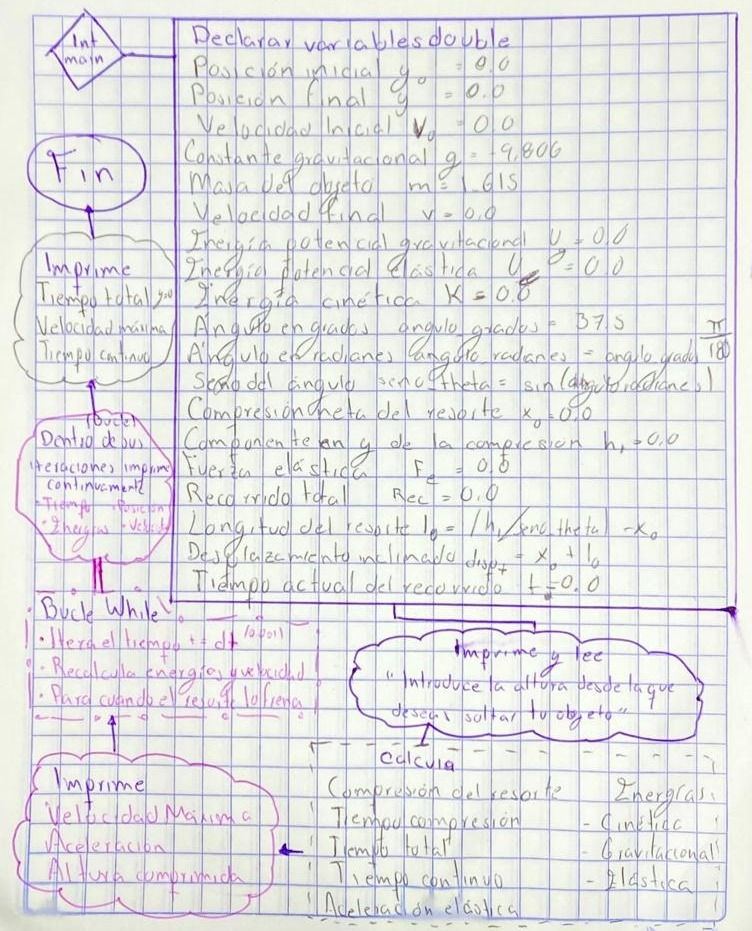
\includegraphics[width=0.8\textwidth]{Diagram.jpeg}
  \caption{Diagrama de flujo para las variaciones energéticas.}
  \label{fig:diagrama}
\end{figure}



\newpage
\section{Pseudocódigo}

\subsubsection*{Configuración inicial}
\begin{align*}
&\text{altura\_inicial} = 0.0 \\
&\text{altura\_final} = 0.0 \\
&\text{velocidad\_inicial} = 0.0 \\
&\text{aceleracion\_gravedad} = -9.808 \\
&\text{masa\_objeto} = 1.615 \\
&\text{velocidad} = 0.0 \\
&\text{energia\_potencial\_gravitacional} = 0.0 \\
&\text{energia\_potencial\_elastica} = 0.0 \\
&\text{energia\_cinetica} = 0.0 \\
&\text{angulo\_grados} = 37.5 \\
&\text{angulo\_radianes} = \text{angulo\_grados} \times \frac{\pi}{180.0} \\
&\text{seno\_theta} = \sin(\text{angulo\_radianes}) \\
&\text{constante\_resorte} = 400.0 \\
&\text{compresion\_resorte} = 0.0 \\
&\text{altura\_compresion} = 0.0 \\
&\text{longitud\_resorte} = \left(\frac{\text{altura\_compresion}}{\text{seno\_theta}}\right) - \text{compresion\_resorte} \\
&\text{desplazamiento\_x} = \text{compresion\_resorte} + \text{longitud\_resorte} \\
&\text{paso\_tiempo} = 0.001 \\
&\text{tiempo\_actual} = 0.0 \\
&\text{recorrido\_total} = 0.0 \\
\end{align*}

\subsubsection*{Entrada de usuario}
\begin{verbatim}
Mostrar("Introduce la altura desde la que deseas soltar tu objeto. [Salto de línea]")
Leer(altura_inicial)
\end{verbatim}

\subsubsection*{Cálculo de la compresión del resorte}
\begin{align*}
&\text{compresion\_resorte} = \sqrt{\frac{m \cdot g \cdot \sin(\theta)^2 + \sqrt{m^2 \cdot g^2 \cdot \sin(\theta)^2 - 4 \cdot 0.5 \cdot k \cdot y_0 \cdot m \cdot g \cdot \sin(\theta)}}{k}} \\
&\text{Si } (\text{altura\_inicial} == 0) \{ \\
&\quad \text{compresion\_resorte} = 0.0 \\
&\} \\
&\text{altura\_compresion} = \frac{0.5 \times \text{constante\_resorte} \times \text{compresion\_resorte}^2}{\text{masa\_objeto} \times \text{aceleracion\_gravedad}} \\
&\text{recorrido\_total} = -\text{altura\_compresion} + \text{altura\_inicial} \\
\end{align*}

\subsubsection*{Cálculo de tiempos y velocidades}
\begin{align*}
&\text{tiempo\_total} = \sqrt{\frac{2 \times \text{recorrido\_total}}{9.806}} \\
&\text{tiempo\_continuo} = \sqrt{\frac{2 \times \text{altura\_inicial}}{9.806}} \\
&\text{tiempo\_compresion\_resorte} = \text{tiempo\_compresion} - \text{tiempo\_continuo} \\
&\text{velocidad\_maxima} = \text{aceleracion\_gravedad} \times \text{tiempo\_continuo} \\
&\text{Mostrar}("\textit{La compresión es [Mostrar 2 decimales]. [Salto de línea] El desplazamiento total es [Mostrar 2 decimales].} \\
&\textit{[Salto de línea]"}, \text{compresion\_resorte}, \text{recorrido\_total}) \\
&\text{aceleracion\_elastica} = \frac{-\text{velocidad\_maxima}}{\text{tiempo\_compresion\_resorte}} \\
&\text{Mostrar("La velocidad máxima es [Mostrar 2 decimales], la aceleración [Mostrar 2 decimales], la altura comprimida es} \\
&\text{[Mostrar 2 decimales], el tiempo de compresión es [Mostrar 2 decimales] [Salto de línea]"},\\
& [Máscara] \text{velocidad\_maxima}, \text{aceleracion\_elastica}, \text{altura\_compresion}, \text{tiempo\_compresion\_res}) \\
&\text{tiempo\_if} = 0.0 \\
\end{align*}

\subsubsection*{Simulación de la caída}
Mientras (altura\_actual $\geq$ altura\_compresion) (\\
    altura\_actual $=$ altura\_inicial + velocidad\_inicial * tiempo\_actual + 0.5 * aceleracion\_gravedad * tiempo\_actual * tiempo\_actual \\
    velocidad $=$ velocidad\_inicial + aceleracion\_gravedad * tiempo\_actual \\
    energia\_potencial\_gravitacional $=$ masa\_objeto * $(-$aceleracion\_gravedad$)$ * altura\_actual \\
    Si (altura\_actual $<$ 0) (\\
        velocidad $=$ velocidad\_maxima + aceleracion\_elastica * tiempo\_if \\
        energia\_potencial\_elastica $=$ 0.5 * constante\_resorte * altura\_actual * altura\_actual * seno\_theta * seno\_theta \\
        tiempo\_if $+=$ paso\_tiempo \\
    ) \\
    energia\_cinetica $=$ 0.5 * masa\_objeto * velocidad * velocidad \\
    Mostrar("[Salto de línea] Tiempo: [Mostrar 3 decimales] segundos, Posición: [Mostrar 3 decimales] m, Velocidad: [Mostrar 3 decimales] m/s, Energía Potencial Gravitacional [Mostrar 3 decimales] J, Energía Cinética [Mostrar 3 decimales] J, Energía Potencial Elástica [Mostrar 3 decimales] J", tiempo\_actual, altura\_actual, velocidad, energia\_potencial\_gravitacional, energia\_cinetica, energia\_potencial\_elastica) \\
    tiempo\_actual $+=$ paso\_tiempo \\
)


Mostrar("[Salto de línea] El tiempo que tardó en llegar al resorte es de [Mostrar 4 decimales] segundos y su velocidad en ese punto [Mostrar 4 decimales]", tiempo\_continuo, velocidad\_maxima)

\textbf{FIN DEL PROGRAMA}

\subsection{Gnuplot instrucciones}

-[Configuración de estilo y etiquetas]\\
set title "Evolución de Energías en el Tiempo"\\
set xlabel "Tiempo (s)"\\
set ylabel "Energía (J)"\\
set key outside\\
set grid\\
\\
-[Graficar las tres líneas del conjunto de datos]\\
plot "datos.dat" using 1:5 with lines title "Energía Cinética" lc rgb 'blue', \\
     "datos.dat" using 1:4 with lines title "Energía Potencial Gravitacional" lc rgb 'green', \\
     "datos.dat" using 1:6 with lines title "Energía Potencial Elástica" lc rgb 'red'\\
\newpage
\section{Programa fuente}
Referido como main.c\\\\

\section{Archivo de datos}
Con magnitud mayor a 200 datos, referido como datos.dat (instrucciones adjuntas en gnuplot instrucciones.txt)\\\\

\section{Gráfica en gnuplot}
Presentada en formato pdf y jpg, en la preferencia del evaluador. Son referidas como "\textit{kinetic, elastic & gravitational energies in the time"} en ambas de sus presentaciones.







\end{document}
